\section{Resultados}

En esta sección se presentan las evidencias obtenidas durante el desarrollo de la práctica, que permiten verificar el correcto funcionamiento del circuito de arranque del motor trifásico.

En primer lugar, se documentó el estado inicial del tablero mediante una fotografía del circuito original, donde se aprecian las conexiones relevadas y los componentes principales del sistema. Posteriormente, se registró en una segunda fotografía el tablero con el cableado completado y verificado, mostrando las modificaciones y correcciones realizadas por el equipo durante el laboratorio (Figura \ref{fig:circuito_completo}).

Para complementar la evidencia visual, se incluye un enlace a un video almacenado en Google Drive donde se observa la secuencia de arranque y detención del motor, junto con la actuación de los contactores y los indicadores luminosos del tablero. Este registro audiovisual constituye una prueba adicional del funcionamiento del sistema bajo condiciones reales de operación:

%\href{https://drive.google.com/tu-enlace}{\textbf{Ver video de funcionamiento}}

Finalmente, en la Tabla \ref{tab:mediciones} se presentan los valores medidos de corriente y potencia eléctrica del motor durante su funcionamiento en régimen permanente. Estos datos fueron obtenidos con pinza amperimétrica y con el instrumento Power Energy Logger, y constituyen la base para el análisis y las conclusiones posteriores.


\begin{figure}[H]
\centering
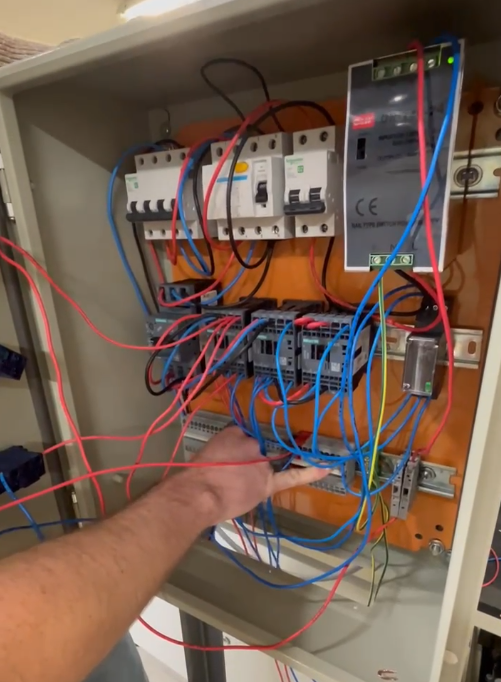
\includegraphics[width=0.4\textwidth]{anexos/circuitoCompleto.png}
\caption{Tablero con el cableado completado y verificado}
\label{fig:circuito_completo}
\end{figure}

\begin{table}[H]
    \centering
    \caption{Corriente medida según la configuración del motor.}

    \begin{tabular}{lc}
        \toprule
        \textbf{Configuración} & \textbf{Corriente (A)} \\
        \midrule
        Estrella (Y)  & 0.039 \\
        Triángulo ($\Delta$) & 0.098 \\
        \bottomrule
    \end{tabular}
\end{table}

%\begin{table}[H]
%\centering
%\caption{Valores de corriente y potencia medidos en el motor trifásico}
%\label{tab:mediciones}
%\begin{tabular}{|c|c|c|}
%\hline
%Fase & Corriente [A] & Potencia [W] \\
%\hline
%L1 & -- & -- \\
%L2 & -- & -- \\
%L3 & -- & -- \\
%\hline
%\end{tabular}
%\end{table}
